\section{Test, test, again ...}
Of course, tweaking the Person List display is not going to be the end of it.
Clients always want more, and now ours wants to edit, add, or delete records.
Let's write some tests for these new tasks, as shown in
Example~\ref{example:9}.

\begin{example}\label{example:9}
New stories, new tests
\begin{verbatim}
    function testPersonUpdate()
    {
        $expect = "wei";
        $edited = "Nah";

        //get it;
        $person = TMapper::instance()->queryForObject("Select", 1);

        //test it
        $this->assertNotNull($person);
        $this->assertEqual($expect, $person->FirstName);

        //change it
        $person->FirstName = $edited;
        TMapper::instance()->update("Update", $person);

        //get it again
        $person = TMapper::instance()->queryForObject("Select", 1);

        //test it
        $this->assertEqual($edited, $person->FirstName);

        //change it back
        $person->FirstName = $expect;
        TMapper::instance()->update("Update", $person);
    }

    function testPersonDelete()
    {
        //insert it
        $person = new Person;
        $person->ID = -1;
        TMapper::instance()->insert("Insert", $person);

        //delte it
        $count = TMapper::instance()->delete("Delete", -1);
        $this->assertEqual(1, $count);
    }
\end{verbatim}
\end{example}

Not the best tests ever written, but for now, they will do :)

To make the new tests work, we'll need some new mapping statements.
Example~\ref{example:10} shows the complete mapper document that we've called
\tt{personHelper.xml}.

\begin{example}
The new and improved mapper document
\begin{verbatim}
<?xml version="1.0" encoding="utf-8" ?>

<sqlMap Name="PersonHelper">
  <select id="Select" parameterClass="int" resultClass="Person">
   select
    PER_ID as ID,
    PER_FIRST_NAME as FirstName,
    PER_LAST_NAME as LastName,
    PER_BIRTH_DATE as BirthDate,
    PER_WEIGHT_KG as WeightInKilograms,
    PER_HEIGHT_M as HeightInMeters
    from PERSON
    WHERE
      PER_ID = #value#
  </select>

  <insert id="Insert" parameterClass="Person">
   insert into PERSON
    (PER_ID, PER_FIRST_NAME, PER_LAST_NAME,
    PER_BIRTH_DATE, PER_WEIGHT_KG, PER_HEIGHT_M)
   values
    (#ID#, #FirstName#, #LastName#,
    #BirthDate#, #WeightInKilograms#, #HeightInMeters#)
  </insert>

  <update id="Update" parameterClass="Person">
   update PERSON set
    PER_FIRST_NAME = #FirstName#,
    PER_LAST_NAME = #LastName#,
    PER_BIRTH_DATE = #BirthDate#,
    PER_WEIGHT_KG = #WeightInKilograms#,
    PER_HEIGHT_M = #HeightInMeters#
   where PER_ID = #ID#
  </update>

  <delete id="Delete" parameterClass="int">
   delete from PERSON
   where PER_ID = #value#
  </delete>
</sqlMap>
\end{verbatim}
\end{example}
Well, waddya know, if run our tests now, we are favored with a green bar!. It
all works!

\begin{mybox}{Note:}
Though, of course, things usually do not work perfectly the first time! We
have to fix this and that, and try, try, again. But SimpleTest makes trying
again quick and easy. You can changes to the XML mapping documents and rerun
the tests! No muss, no fuss.
\end{mybox}

Turning back to our Prado page, we can revamp the TDataGrid to allow in-place
editing and deleting. To add records, we provide a button after the grid that
inserts a blank person for client to edit. The page code is shown as
Example~\ref{example:11}.
\begin{example}\label{example:11}
Prado page code for our enhanced TDataGrid
\begin{verbatim}
    <com:TDataGrid id="personList"
            DataKeyField="ID"
            AutoGenerateColumns="False"
            OnEditCommand="editPerson"
            OnUpdateCommand="updatePerson"
            OnCancelCommand="refreshList"
            OnDeleteCommand="deletePerson">
        <com:TBoundColumn DataField="FirstName" HeaderText="First Name" />
        <com:TBoundColumn DataField="LastName" HeaderText="Last Name" />
        <com:TBoundColumn DataField="HeightInMeters" HeaderText="Height" />
        <com:TBoundColumn DataField="WeightInKilograms" HeaderText="Weight" />
        <com:TEditCommandColumn
                HeaderText="Edit"
                UpdateText="Save" />
        <com:TButtonColumn
                HeaderText="Delete"
                Text="Delete"
                CommandName="delete"/>
    </com:TDataGrid>
    <com:TButton Text="Add" OnClick="addNewPerson" />
\end{verbatim}
\end{example}

Example~\ref{example:12} shows the corresponding methods from page PHP class.

\begin{example}\label{example:12}
The page class code for our enhanced TDataGrid
\begin{verbatim}
    private function sqlmap()
    {
        return $this->Application->getModule('SQLMap')->getClient();
    }

    private function loadData()
    {
        $this->personList->DataSource =
                $this->sqlmap()->queryForList('SelectAll');
        $this->personList->dataBind();
    }

    public function onLoad($param)
    {
        if(!$this->IsPostBack)
            $this->loadData();
    }

    protected function editPerson($sender,$param)
    {
        $this->personList->EditItemIndex=$param->Item->ItemIndex;
        $this->loadData();
    }

    protected function deletePerson($sender, $param)
    {
        $id = $this->getKey($sender, $param);
        $this->sqlmap()->update("Delete", $id);
        $this->loadData();
    }

    protected function updatePerson($sender, $param)
    {
        $person = new Person();
        $person->FirstName = $this->getText($param, 0);
        $person->LastName = $this->getText($param, 1);
        $person->HeightInMeters = $this->getText($param, 2);
        $person->WeightInKilograms = $this->getText($param, 3);
        $person->ID = $this->getKey($sender, $param);
        $this->sqlmap()->update("Update", $person);
        $this->refreshList($sender, $param);
    }

    protected function addNewPerson($sender, $param)
    {
        $person = new Person;
        $person->FirstName = "-- New Person --";
        $this->sqlmap()->insert("Insert", $person);
        $this->loadData();;
    }

    protected function refreshList($sender, $param)
    {
        $this->personList->EditItemIndex=-1;
        $this->loadData();
    }

    private function getText($param, $index)
    {
        $item = $param->Item;
        return $item->Cells[$index]->Controls[0]->Text;
    }

    private function getKey($sender, $param)
    {
        return $sender->DataKeys[$param->Item->DataSourceIndex];
    }
\end{verbatim}
\end{example}

OK, we are CRUD complete! There's more we could do here. In particular, we
should add validation methods to prevent client from entering alphabetic
characters where only numbers can live. But, that's a different Prado
tutorial, and this is an SQLMap DataMapper tutorial.

\begin{figure}[!h]
    \centering
        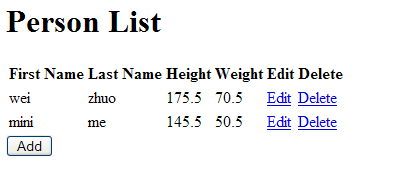
\includegraphics[width=0.75\textwidth]{grid2}
    \caption{Person List CRUD}
    \label{figure:2}
\end{figure}
